\section{Motivation} \label{motivation-l}
DNA methylation is a well studied chemical modification of DNA, which occurs when a methyl group is attached to a DNA nucleotide. It is associated with diverse biological processes of direct clinical relevance, including gene and transposon silencing, X-chromosome inactivation, and  genomic imprinting \citep{Li1993, Mohandas1981}. In mammals,  methylation is observed almost exclusively on cytosine residues in the context of CpG dinucleotides (\ie C followed by G, where p stands for the phosphate group linking C and G). DNA methylation is said to be a true \emph{epigenetic modification}, since its mechanism of inheritance during the cell cycle is well established \citep{Law2010}. 

Due to the increased vulnerability of the 5-methylcytosines to randomly deaminate to thymine, most of the genome is depleted from CpG dinucleotides \citep{Scarano1967}, except from small regions termed \emph{CpG islands} \citep{Bird2002}. A CpG island (CGI) is a sequence of at least 200 bp with a greater number of CpG sites than expected from its GC content. These regions are often GC rich, typically undermethylated, and are found upstream of many mammalian genes \citep{Law2010}. 

Bisulphite treatment \citep{Frommer1992} followed by next generation sequencing (NGS) can be used to measure the methylation level of the genomic DNA at a single-nucleotide resolution, and is termed Whole-Genome Bisulphite Sequencing (WGBS). Sodium bisulphite efficiently deaminates unmethylated cytosines to uracils, and leaves the 5-Methylcytosines unchanged. Uracils are read as thymines by DNA polymerase, thus when amplifying the data during PCR, the unmethylated cytosines appear as thymines \citep{Krueger2012}. Reads are then aligned to a reference genome allowing changes of C to T during the mapping procedure. 

The outline of the bisulphite treatment of a sample DNA sequence is shown in \emph{Figure \ref{bisulphite-pic}}.

\begin{figure}[!h]
	\begin{center}
 		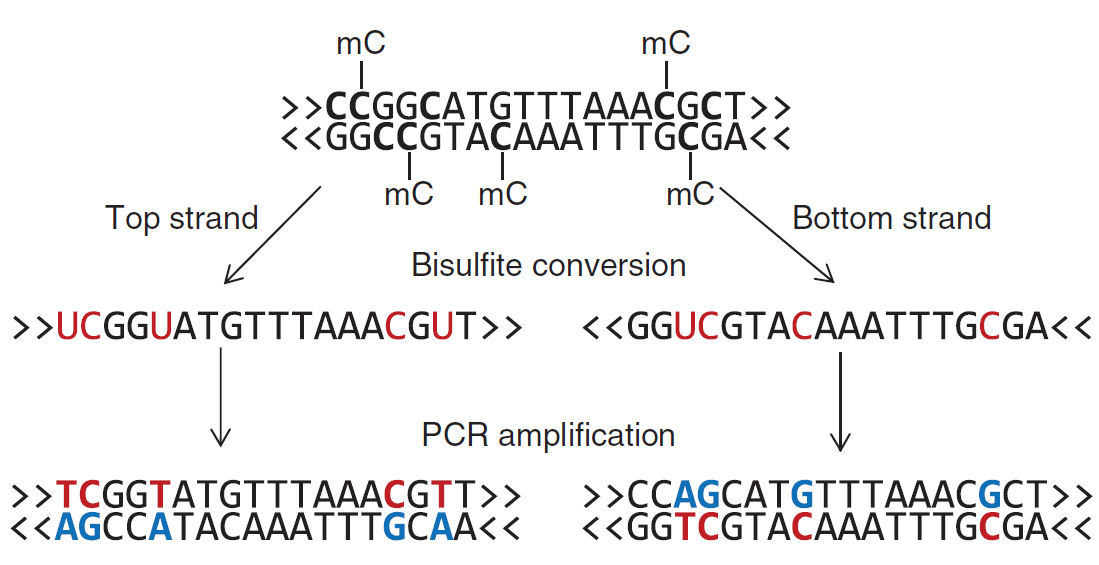
\includegraphics[scale = 0.43]{images/bis-treatment.png}
		\caption{\emph{Outline of the bisulphite treatment and subsequent PCR amplification of a sample DNA sequence. Unmethylated cytosines are deaminated to uracils by bisulphite, while 5-Methylcytosines are resistant to conversion \citep{Krueger2012}.}}
		\label{bisulphite-pic}
	\end{center}
\end{figure} 

In WGBS experiments, the DNA molecules often originate from distinct cells, as a consequence, the methylation state of a particular cytosine may be different across DNA molecules. Hence, in the context of WGBS experiments the methylation of a particular cytosine is described as \emph{methylation level}, which is the fraction of the molecules in the sample containing 5-Methylcytosine at the specific genomic locus \citep{Schultz2012}. \emph{Read coverage} is the average number of times a CpG site is read during the sequencing process, and this depends on the depth of the sequencing.

\cite{Meissner2005} developed a technique, termed Reduced Representation Bisulfite Sequencing (RRBS), for analyzing the genome-wide methylation profiles efficiently, at lower cost and with greater coverage of CpG dense regions. This method, combines bisulphite treatment and restriction enzymes, such as MspI, to generate a 'reduced representation' of the genome of a strain, tissue or cell type which have a high CpG content \citep{Meissner2005}. 

What is often of practical interest is identifying the methylation profile of a genomic region, \eg the methylation profile of a promoter. \cite{Vanderkraats2013} suggested that the shape of the methylation profile plays an important role in predicting gene expression, leading to a potentially functional role for methylation patterns. This means that higher-order properties, such as shape, of the methylation profiles over a region should be considered. Taking into consideration that the methylation level of a CpG site is highly correlated with the methylation level of the surrounding CpGs (\ie spatial co-dependence), \cite{Mayo2014} developed M$^3$D, which is non-parametric kernel-based method for statistical identification of differentially methylated regions (DMRs). This project makes the same assumption about the \emph{spatial co-dependence} of CpGs, but is mainly concentrated in clustering together similar methylation profiles.



\section{Modelling DNA methylation profiles} \label{model-meth-profiles-s}
DNA methylation data generated from next generation sequencing methods can be modelled with a Binomial distribution. Assume that \emph{t} is the total number of reads that are mapped to a specific CpG site, and that the 5-Methylcytosine were found in \emph{m} of these reads. Then for each CpG cite we have the read proportion \emph{(m,t)}, and we assume that:
\begin{equation} \label{binom-1d-f}
	m \sim Binom(t, p)
\end{equation}

where \emph{p} is the unknown methylation level of the CpG site.

We are interested in modelling methylation profiles across different genomic regions, \eg promoter regions, hence the data can be represented as a set of vectors, whose dimensionality \emph{L} depends on the number of the individual CpG sites for that specific region. Thus, each region \emph{i} can be represented by a vector $\mathbf{y}_{i}$ of dimensionality $L_{i}$, and each entry of the vector consists of the tuple:
\begin{equation}
	%n_{i}^{l} = \frac{m_{i}^{l}}{t_{i}^{l}}
	y_{il} = (m_{il},t_{il})
\end{equation}

where, $m_{il}$ is the number of 5-Methylcytosine reads on $l$-th CpG site in region $i$, and $t_{il}$ is the total number of reads on $l$-th CpG site in region $i$. 

Thus, we can formulate our problem as a \emph{regression} problem, where we try to fit a function $\mathbf{f}$, of some specific form, to the observations $\mathbf{y}$. A promising approach for modelling the methylation profile for a given region is to use a \emph{Gaussian Process} for classification \citep{Rasmussen2006}. Even though this approach would be ideal, its time complexity of $O(n^{3})$ is prohibitive for our purposes. Thus, we have to resort in modelling the methylation level using $n^{th}$ degree polynomial functions.

More specifically, let $\mathbf{x}_{i}$ be the genomic region of interest, $\mathbf{y}_{i}$ be the observations in this region (\ie proportions of methylated reads to the total reads at each site), and let $f(\mathbf{x}_{i})$ be a latent function representing the methylation profile at that specific genomic region. Since the methylation data take values in the $[0, 1]$ interval, we introduce a latent function $g(\mathbf{x}_{i})$, \eg $g(\mathbf{x}_{i}) = \alpha \mathbf{x}_{i}^{2} + \beta \mathbf{x}_{i} + c$, defined as the \emph{inverse probit transformation} of $f(\mathbf{x}_{i})$. In other words, $f(\mathbf{x}_{i})$ is the probit transformation of $g(\mathbf{x}_{i})$:
\begin{equation} \label{probit-transform-f}
	f(\mathbf{x}_{i}) = \Phi(g(\mathbf{x}_{i}))
\end{equation}

where $\Phi(x)$ is the Cumulative Distribution Function (CDF) of the standard normal distribution:
\begin{equation} \label{cdf-stand-normal-f}
	\Phi(x) = \frac{1}{\sqrt{2\pi}} \int_{-\infty}^{x} e^{-t^{2}/2}dt
\end{equation}

Let $\mathbf{f}_{i} = f(\mathbf{x}_{i})$ and $\mathbf{g}_{i} = g(\mathbf{x}_{i})$ be shorthand for the values of the latent functions.

Given the values of the latent function $\mathbf{f}_{i}$, the observations at each CpG site for that region are independent Binomial variables, as shown in \emph{Eq. \ref{binom-1d-f}}, so the joint likelihood factorizes and we have:
\begin{equation} \label{likel-binom-prob-f}
  \begin{split}
	p(\mathbf{y}_{i}|\mathbf{f}_{i}) & = \prod_{l=1}^{L} p(y_{il}|f_{il}) \\
							 & = \prod_{l=1}^{L} Binom(t_{il}, f_{il}) \\
							 & = \prod_{l=1}^{L} Binom\big(t_{il}, \Phi(g_{il})\big) \\
							 & = \prod_{l=1}^{L} \binom{t_{il}}{m_{il}} \Phi(g_{il})^{m_{il}} (1 - \Phi(g_{il})\big)^{t_{il} - m_{il}}
  \end{split}
\end{equation}

From its final form, we refer to this function as the Binomial distributed Probit regression function. In practice, the likelihood is computed in the log space, due to numerical issues when multiplying many probabilities of small numbers leading to underflow errors. Thus, the joint log likelihood for region \emph{i} is:
\begin{equation} \label{likel-binom-prob-log-f}
  \begin{split}
	\log p(\mathbf{y}_{i}|\mathbf{f}_{i}) & = \sum_{l=1}^{L} \log p(y_{il}|f_{il}) \\
				& = \sum_{l=1}^{L} \log \bigg(\binom{t_{il}}{m_{il}} \Phi(g_{il})^{m_{il}} \big(1 - \Phi(g_{il})\big)^{t_{il} - m_{il}}\bigg) \\
				& = \sum_{l=1}^{L} \bigg(\log \binom{t_{il}}{m_{il}} + m_{il} \log \Phi(g_{il}) + \big(t_{il} - m_{il} \big) \big(1 - \Phi(g_{il})\big)\bigg)
  \end{split}
\end{equation}


\section{Clustering DNA methylation profiles}
The main aim of this project is focused on clustering multisource biomedical data. Thus, after defining a model for methylation profiles, a statistical method needs to be proposed in order to perform model-based clustering of DNA methylation profiles.

The most widely used approach for clustering data, and the one that is taken in this project, is to use a \emph{mixture model} \citep{McLachlan1988}. A mixture model is a convex combination of two or more probability density functions, possibly of different distributional types. By using a superposition of the individual probability density functions, mixture models are capable of approximating any continuous distribution to arbitrary accuracy \citep{Marin2005}. Mixture models can be formulated as Latent Variable Models (LVMs), where the latent variables have discrete states and can be interpreted as defining assignments of data points to specific components of the mixture model.

Formally, let $X_{i}$, where $i \in \lbrace 1, ... , N \rbrace$, be a given dataset with N objects. The goal of clustering is to partition the objects into at most K clusters. Let $p(X_{i}|\theta)$ be the probability distribution for $X_{i}$ parametrized by $\theta$, $C_{i} \in \lbrace 1,...,K \rbrace$ represent the  component that is responsible for $X_{i}$, and $\pi_{k}$ be the probability that an object belongs to cluster $k$, i.e. $\pi_{k} = P(C_{i} = k)$. 

Thus, the mixture model is defined as follows:
\begin{equation}
	\begin{aligned}
		& 
		& & p(X_{i}|\Theta) = \sum_{k=1}^{K}\pi_{k}p(X_{i}|\theta_{k}) \\
		& where 
		& & \pi_{k} \in (0, 1) \forall k, \; \sum_{k=1}^{K}\pi_{k} = 1  \; \text{and} \; \Theta = (\theta_{1},...,\theta_{k})
	\end{aligned}
\end{equation}

\subsection{Expectation Maximization algorithm}
The model can be fitted to the data using maximum likelihood estimators. For LVMs the standard technique is to use \emph{Expectation Maximization} (EM) algorithm \citep{Dempster1977}. EM is an iterative algorithm, which alternates between computing the expected log likelihood under the posterior distribution of the latent variables using the current estimate of the parameters (\emph{E-step}), and then maximizing the expected log likelihood (\emph{M-step}). The algorithm ends when the convergence criterion is satisfied. Actually EM exploits the fact that if the data were fully observed then the Maximum Likelihood Estimate (MLE) would be easy to compute. In their classic paper \cite{Dempster1977} proved that EM monotonically increases the log likelihood and it converges to a maximum likelihood estimator. 

Our presentation for the derivation of the EM algorithm is based on \cite[Ch. \ 11]{Murphy2012}.

Let $x_{i}$ be the observed variables, and $z_{i}$ be the hidden or latent variables. We are interested in maximizing the log likelihood of the observed data:
\begin{equation} \label{log-lik-observed-f}
	\ell(\theta) \triangleq \sum_{i=1}^{N} \log p(x_{i}|\theta) =  \sum_{i=1}^{N} \log \bigg[\sum_{z_{i}} p(x_{i}, z_{i}|\theta) \bigg]
\end{equation}

which is hard to optimize due to the presence of the summation inside the logarithm, so the logarithm no longer acts directly on the likelihood function.

Let us define the \emph{complete data log likelihood} as follows:
\begin{equation} \label{log-lik-observed-f}
	\ell_{c}(\theta) \triangleq \sum_{i=1}^{N} \log p(x_{i}, z_{i}|\theta)
\end{equation}

If the variables $z_{i}$ were observed, we assume that this likelihood could be easily computed. EM gets around with this problem by defining the \emph{expected complete data log likelihood} as:
\begin{equation} \label{log-lik-expected-f}
		Q(\theta, \theta^{t-1}) \triangleq \mathbb{E} \big[\ell_{c}(\theta) | D, \theta^{t-1}\big]
\end{equation}

where $t$ is the current iteration. The expectation is taken with respect to the old parameters $\theta^{t-1}$ and the observed data $D$. In the E-step, we compute the terms inside $Q(\theta, \theta^{t-1})$ which MLE depends on. In the M-step, we optimize Q with respect to $\theta$:
\begin{equation} \label{log-lik-observed-f}
	\theta^{t} = \underset{\theta}{\operatorname{argmax}} \; Q(\theta, \theta^{t-1})
\end{equation}

For the specific case of mixture models, the expected complete data log likelihood is:
\begin{equation} \label{log-lik-expected-f}
	\begin{split}
		Q(\theta, \theta^{t-1}) & \triangleq \mathbb{E} \big[\ell_{c}(\theta) | D, \theta^{t-1}\big] \\
								& = \mathbb{E} \bigg[ \sum_{i} \log p(x_{i}, z_{i}|\theta) \bigg] \\
								& = \sum_{i} \mathbb{E} \bigg[ \log \bigg[\prod_{k} \big( \pi_{k}p(x_{i}|\theta_{k})\big)^{\mathbb{I}(z_{i}=k)} \bigg]\bigg] \\
								& = \sum_{i} \sum_{k} \mathbb{E} \big[\mathbb{I}(z_{i}=k)\big] \log \big[\pi_{k}p(x_{i}|\theta_{k})\big] \\
								& = \sum_{i} \sum_{k} p(z_{i}=k|x_{i},\theta^{t-1}) \log \big[\pi_{k}p(x_{i}|\theta_{k})\big] \\
								& = \sum_{i} \sum_{k} \gamma(z_{ik}) \log \big[\pi_{k}p(x_{i}|\theta_{k})\big] \\
								& = \sum_{i} \sum_{k} \gamma(z_{ik}) \log \pi_{k} + \sum_{i} \sum_{k} \gamma(z_{ik}) \log p(x_{i}|\theta_{k}) \\		
	\end{split}
\end{equation}

where, $\gamma(z_{ik}) \triangleq p(z_{i}=k|x_{i},\theta_{k}^{t-1})$ is the responsibility that component k takes for explaining the observation $x_{i}$, and $\mathbb{I}(z_{i}=k)$ is an indicator function, equal to 1 if $z_{i}=k$, and 0 otherwise.

\noindent
\textbf{E-step}: The E-step can be computed using the following form for any mixture model:
\begin{equation} \label{responsibilities-f}
  \begin{split}
	\gamma(z_{ik}) & \triangleq p(z_{i}=k|x_{i},\theta_{k}^{t-1}) \\
				   & = \frac{p(z_{i}=k)p(x_{i}|z_{i}=k,\theta_{k}^{t-1})}{\sum\limits_{j=1}^{K} p(z_{i}=j)p(x_{i}|z_{i}=j,\theta_{j}^{t-1})} \\
				   & = \frac{\pi_{k}p(x_{i}|z_{i}=k,\theta_{k}^{t-1})}{\sum\limits_{j=1}^{K} \pi_{j}p(x_{i}|z_{i}=j,\theta_{j}^{t-1})}
  \end{split}
\end{equation}

\noindent
\textbf{M-step}: In the M-step we optimize $Q$ with respect to $\pi_{k}$ and the parameters $\theta_{k}$.

For the mixing proportions $\pi_{k}$, we take the derivative of \emph{Eq. \ref{log-lik-expected-f}} wrt $\pi_{k}$ and set it to zero, also due to the constraint that $\sum_{k=1}^{K}\pi_{k} = 1$ we introduce a Langrange multiplier. The result, which is the same for any mixture model, is:
\begin{equation} \label{mixing-proportions-est-f}
		\pi_{k} = \frac{1}{N} \sum_{i} \gamma(z_{ik})
\end{equation}

To derive the M-step for the parameters $\theta_{k}$, we only keep the terms of \emph{Eq. \ref{log-lik-expected-f}} that depend on $\theta_{k}$, that is:
\begin{equation} \label{parameters-est-EM-f}
		\ell(\theta_{k}) \triangleq \sum_{i} \sum_{k} \gamma(z_{ik}) \log p(x_{i}|\theta_{k})
\end{equation}

and we optimize them with respect to $\theta_{k}$.

The maximization of \emph{Eq. \ref{parameters-est-EM-f}} yields different results depending on the likelihood function $p(x_{i}|\theta_{k})$. For most of the well known probability distributions, including the Normal, Binomial, Poisson, etc., the maximization of $\ell(\theta_{k})$ is feasible. 

For more complex likelihood functions, the maximization of $\ell(\theta_{k})$ may be intractable, thus numerical optimization strategies \citep{Nocedal2006}, such as conjugate gradients algorithm \citep{Hestenes1952} should be exploited. This extension of EM algorithm is known as \emph{Generalised EM}, or GEM, and it has been proved that on each EM iteration of the GEM algorithm the log likelihood increases, and thus converges to the maximum likelihood estimator \citep{Wu1983}.

\subsection{EM for clustering methylation profiles}
In this section, we will derive the \emph{E} and \emph{M} steps for clustering methylation profiles using the model described in \emph{Section \ref{model-meth-profiles-s}}.

But before we have to explicitly introduce the parameters $\theta_{k}$ of the model, excluding the mixing proportions $\pi_{k}$ which are present for any mixture model. For example, in a Gaussian Mixture Model (GMM) the model parameters $\theta_{k}$, are the mean $\mu_{k}$ and the variance $\sigma_{k}^{2}$ of the Gaussian components. In our model, the Binomial distributed Probit regression function given in \emph{Eq. \ref{likel-binom-prob-f}}, the parameters are the coefficients of the $n^{th}$ degree polynomial function $\mathbf{g}_{i}$. Thus, during the EM algorithm we infer these sets of parameters for each cluster $k$. For example, for a $2^{nd}$ degree polynomial, we can rewrite \emph{Eq. \ref{likel-binom-prob-f}} by explicitly showing the model parameters as follows:
\begin{equation} \label{likel-binom-prob-example1-f}
  \begin{split}
	p(\mathbf{y}_{i}|\mathbf{f}_{i}, \theta) & = \prod_{l=1}^{L} p(y_{il}|f_{il}, \theta) \\
							 & = \prod_{l=1}^{L} Binom \big(t_{il}, \Phi(g_{il}; \theta)\big) \\
							 & = \prod_{l=1}^{L} \binom{t_{il}}{m_{il}} \Phi(\alpha x_{il}^{2} + \beta x_{il} + c)^{m_{il}} (1 - \Phi(\alpha x_{il}^{2} + \beta x_{il} + c)\big)^{t_{il} - m_{il}}
  \end{split}
\end{equation}

where $\theta = (\alpha, \beta, c)$.

\subsubsection{E-Step}
In the E-step we compute the responsibility that component k takes on explaining observations $\mathbf{y_{i}}$, and by substituting the proposed likelihood function to \emph{Eq. \ref{responsibilities-f}}, we have:
\begin{equation} \label{responsibilities-model-f}
  \begin{split}
	\gamma(z_{ik}) & \triangleq p(z_{i}=k|\mathbf{y_{i}},\theta_{k}^{t-1}) \\
				   & = \frac{\pi_{k}p(\mathbf{y}_{i}|\mathbf{f}_{i},z_{i}=k,\theta_{k}^{t-1})}{\sum\limits_{j=1}^{K} \pi_{j}p(\mathbf{y}_{i}|\mathbf{f}_{i},z_{i}=j,\theta_{j}^{t-1})} \\
				   & = \frac{\pi_{k} \prod\limits_{l=1}^{L} Binom \big(t_{il}, \Phi(g_{il}; \theta_{k}^{t-1})\big)} {\sum\limits_{j=1}^{K} \pi_{j} \prod\limits_{l=1}^{L} Binom \big(t_{il}, \Phi(g_{il}; \theta_{j}^{t-1})\big)}
  \end{split}
\end{equation}

\subsubsection{M-Step}
In the M-step, we optimize \emph{Eq. \ref{log-lik-expected-f}} with respect to $\pi_{k}$ and $\theta_{k}$. The update for the mixing proportions $\pi_{k}$ on each M-step, is the same as shown in \emph{Eq. \ref{mixing-proportions-est-f}}, that is:
\begin{equation} \label{mixing-proportions-est2-f}
		\pi_{k} = \frac{1}{N} \sum_{i} \gamma(z_{ik})
\end{equation}

To update the parameters $\theta_{k}$, we need to optimize $\ell(\theta_{k})$. Substituting our model to \emph{Eq. \ref{parameters-est-EM-f}}, the quantity that needs to be maximized is:
\begin{equation} \label{parameters-est2-EM-f}
  \begin{split}
	\ell(\theta_{k}) & \triangleq \sum_{i} \sum_{k} \gamma(z_{ik}) \log p(\mathbf{y}_{i}|\mathbf{f}_{i}, \theta_{k}) \\
					 & = \sum_{i} \sum_{k} \gamma(z_{ik}) \log \bigg( \prod_{l} Binom \big(t_{il}, \Phi(g_{il}; \theta_{k})\big) \bigg)\\
					 & = \sum_{i} \sum_{k} \gamma(z_{ik}) \sum_{l} \log \bigg(Binom \big(t_{il}, \Phi(g_{il}; \theta_{k})\big) \bigg)
  \end{split}
\end{equation}

Direct maximization of this quantity w.r.t the parameters $\theta_{k}$ is not feasible, thus Conjugate Gradients method \citep{Hestenes1952} will be used, which is a first order numerical optimization algorithm for solving particular systems of linear equations. Thus, it requires to compute the \emph{gradient}:

\begin{equation} \label{gradient-f}
	\nabla\ell = \bigg( \frac{\partial \ell(\theta_{k})}{\partial \alpha}, \frac{\partial \ell(\theta_{k})}{\partial \beta}, \frac{\partial \ell(\theta_{k})}{\partial c}\bigg) 
\end{equation}

where the partial derivatives are given in the equations below (see Appendix ... for the whole derivations):
\begin{equation} \label{derivative-a-f}
	\frac{\partial \ell(\theta_{k})}{\partial \alpha} =  \sum_{i}  \gamma(z_{ik}) \sum_{l} \bigg[ x_{il}^{2} \mathbf{\phi}(g_{il};\theta_{k})\bigg(\frac{m_{il} - t_{il}\Phi(g_{il};\theta_{k})}{\Phi(g_{il};\theta_{k})\big(1-\Phi(g_{il};\theta_{k})\big)} \bigg) \bigg]
\end{equation}

\begin{equation} \label{derivative-b-f}
	\frac{\partial \ell(\theta_{k})}{\partial \beta} =  \sum_{i}  \gamma(z_{ik}) \sum_{l} \bigg[ x_{il} \mathbf{\phi}(g_{il};\theta_{k})\bigg(\frac{m_{il} - t_{il}\Phi(g_{il};\theta_{k})}{\Phi(g_{il};\theta_{k})\big(1-\Phi(g_{il};\theta_{k})\big)} \bigg) \bigg]
\end{equation}

\begin{equation} \label{derivative-c-f}
	\frac{\partial \ell(\theta_{k})}{\partial c} =  \sum_{i}  \gamma(z_{ik}) \sum_{l} \bigg[ \mathbf{\phi}(g_{il};\theta_{k})\bigg(\frac{m_{il} - t_{il}\Phi(g_{il};\theta_{k})}{\Phi(g_{il};\theta_{k})\big(1-\Phi(g_{il};\theta_{k})\big)} \bigg) \bigg]
\end{equation}

where $\mathbf{\phi}$ is the \emph{probability density function (pdf)} for the standard normal distribution $\mathcal{N}(0,1)$.